% vm.tex
\chapter{虚拟内存管理}\label{ch_vm}

\section{本章概要}

\paragraph{一句话描述}
在现代计算系统中,软件所在的代码和数据都是在内存中处理的,操作系统需要管理好内存,让代码和数据能够合理放置在相关位置;且通过提供动态申请内存和释放内存的功能,让自己和依靠操作系统的应用能够灵活高效地使用内存。


\paragraph{概述}

一个编程人员希望拥有容量无限大、速度无限快,而且是非易失型的(nonvolatile)的内存空间,到lab1为止,这个梦想还无法轻易满足。为此绝大多数的计算机采用了一种折衷的方法,即建立一个分层的存储器结构,最高层是CPU内部的一些寄存器,它们的访问速度是最快的,但容量不是很大,一般小于1KB;第二层是高速缓存(即硬件cache),实现在CPU内部,接近寄存器速度,容量一般小于4MB;第三层是主存储器(内存),其访问速度比寄存器小一个数量级、价格便宜,目前几百块人民币就可以买到4GB。以上这三种存储器都是易失型的,即在断电后,其内容全部会丢失掉。第四层是磁盘,它的访问速度较慢、价格较便宜,目前花几百块钱就可以买到存储容量\textgreater{}1TB的硬盘,而且是非易失型的。

操作系统需要尽量满足编程人员的梦想,为此它需要管理上述存储器层次结构形成的存储空间,并完成如下主要任务:

\begin{itemize}
	\item
	记录存储空间的使用情况,即记录哪些部分正在被使用,哪些部分还空闲;
	\item
	当需求方需要存储空间时,能快速地分配给它合适大小的空间;在需求方显式表示不需要申请到的存储空间时,能把存储空间回收,便于以后的分配;
	\item
	隔离不同的内存区域,确保在限制在一个内存区域中运行的软件无法访问区域以外的内存空间。这种机制称为地址保护(地址隔离)机制。
	\item
	如果内存太小,就需要把内存当中使用较少的数据所占空间送到磁盘上,给使用较多的数据腾出内存空间来;如果将来又访问到缓存到硬盘的数据,需要把这些数据重新加载到内存中进行访问。这种机制称为换入换出(swap
	in/out)机制,并涉及页替换算法。
	\item
	即使需求方表明了需要内存,但如果需求方没有实际访问所需内存前,则并不完成实际的物理内存分配。这种机制称为按需分配(如果是基于很分页机制,也称为按需分页)。
	\item
	设两个具有父子关系的程序共享同一地址空间(子程序同享父程序的地址空间),若二程序只是读此地址空间,则地址空间不会有变化;若其中一个程序对此地址空间某地址进行了写操作,则要把包含此地址的页空间复制一份给执行写操作的程序,这时此二程序将有不同的地址空间,可独立运行,相互不干扰。这种机制减少了父程序创建子程序地址空间的开销,称为写时复制(Copy
	On Write,简称COW)机制。
\end{itemize}

\paragraph{本章涉及的实验}

本章内容主要涉及操作系统的内存管理,包括物理内存管理和基于分页机制的虚拟内存管理。读者通过阅读本章的内容并动手实践相关的5个project实验:

\begin{itemize}
	\item
	proj5:能够探测物理内存并建立页表,实现分页管理
	\item
	proj5.1/5.1.1/5.1.2:实现基于连续物理页的first/best/worst-fit分配算法
	\item
	proj5.2:实现基于连续物理页的buddy分配算法
	\item
	proj6:实现任意大小内存分配的slab分配算法
	\item
	proj7:实现缺页中断服务例程和虚拟内存管理结构(VMM
	struct),提供按需分页的支持
	\item
	proj8:实现类似改进时钟算法的页面置换算法并支持页粒度的换入换出机制
	\item
	proj9/proj9.1/proj9.2:完善虚存管理(proj9)并逐步实现了进程间内存共享(proj9.1)和copy
	on write(COW)机制(proj9.2)
\end{itemize}



\paragraph{本章收获的知识}

\textbf{可以掌握如下知识:} * 与操作系统原理相关 *
内存管理:基于分页机制的内存管理 * 内存管理:连续内存分配算法 *
内存管理:非连续内存分配算法 * 内存管理和中断:缺页中断服务例程 *
内存管理:虚存管理中的页面置换算法和页换入换出机制 *
内存管理:按需分页机制和写时复制机制 * 操作系统原理之外 *
80386对分页管理(页表等)的硬件支持 *
页粒度的页面置换策略和页换入换出的具体实现

本章内容中主要涉及内存管理的重要功能主要有两个:

\begin{itemize}
	\item
	提供空闲内存空间:这样给操作系统和应用程序的代码和数据足够的存放``地方'',使得二者能够正常高效地运行,为此需要完成内存/外存的空间的分配、管理、释放等算法。
	\item
	提供内存空间隔离保护:隔离用户态应用程序和内核态操作系统之间,以及不同应用程序之间的内存空间,使得不会出现访问冲突,为此需要为不同的应用程序和操作系统划分不同的地址空间,一个应用程序越界规定的地址空间会出现内存访问故障中断。
\end{itemize}

为了让读者能够从实践上来理解内存管理的基本原理,我们设计了上述实验,主要的功能逐步实现如下所示:
* 首先是扩展ucore的功能,使它能够发现并管理PC系统中可用的空闲物理内存;
*
然后是建立分页机制,建立线性地址(分段机制已经完成了逻辑地址到线性地址的转换)到物理地址的映射关系和具体转换操作,这样使得应用程序无法直接访问到物理地址,而是只能访问由操作系统设定好的物理地址空间,从而使得应用程序的访问空间可控;
*
为了高效地完成操作系统的其他功能单元和应用程序的空闲内存空间需求,需要设计以页(4096字节)为最小分配单位的面向连续物理地址空间的内存分配算法;
还要设计面向任意大小的内存空间(在物理地址空间上不一定连续)的虚拟内存分配算法;
*
为了给应用程序提供超过实际物理内存空间大小的虚拟内存空间,需要把临时不常用到的内存换出(swap
out)到硬盘(也称外存)中,等到需要访问的时候,再换入(swap
in)到内存中。设计高效的页面置换算法会尽量保存经常访问的数据在内存中,而不经常访问的数据会换出到硬盘中。

\section{实现虚存管理功能}\label{ux5b9eux73b0ux865aux5b58ux7ba1ux7406ux529fux80fd}

\subsection{试验目标}\label{ux8bd5ux9a8cux76eeux6807}

有了页表的支持,我们可以使得不同用户态运行程序的内存空间之间无法访问,达到隔离和保护的作用。但页表如何仅仅只支持这个功能就太大材小用了。我们其实还可以通过页表实现更多的功能:

\begin{itemize}
\item
  内存共享:把两个虚拟地址空间通过页表映射到同一物理地址空间。这只需通过设置不同索引的页表项的内容一致即可。
\item
  提供超过物理内存大小的虚拟内存空间:这一步需要结合异常中断处理和硬盘来完成。其基本思想是在内存中放置最常用的一些数据,不常用的数据会被放到硬盘上,但给用户态的软件一种感觉,觉得这些数据都在内存中。当用户态软件访问到的数据不在内存中(暂时存放在硬盘上)的时候,这条访存指令会引发异常中断,由操作系统的异常中断处理例程进行管理。这时操作系统会分析引发异常的内存地址,能够把对应缓存在硬盘中的数据重新读入这个内存地址,并让用户态软件重新执行产生访存异常的那条指令。这些由操作系统完成的工作在用户态完全``看''不到。从用户态软件的角度看,只是操作系统给用户提供了一个超出实际物理内存大小的虚拟内存空间。
\item
  按需分配内存:用户态软件在运行时要求操作系统提供很大的内存,操作系统``表面上''表示满足用户需求,但在背后并没有实际分配对应的物理内存空间。等到用户态软件实际执行到对这些内存的访问时,由于没有分配对应的物理内存空间,会导致产生访存异常。操作系统的异常中断处理例程发觉这是用户态软件以前确实要求过的内存空间,则在从系统管理的空闲空间中分配一页或几页物理内存给用户态软件,并让用户态软件重新执行产生访存异常的那条指令。这些由操作系统完成的工作在用户态也完全``看''不到。但从操作系统的整体管理的角度看,这种方式在用户态软件确实需要的时候把内存分配给用户态软件,提高了内存的使用率,避免了用户态软件``圈地不用''的现象。
\end{itemize}

为了高效地完成上述三件事情,操作系统需要考虑应该把哪些不常用的内存换出到硬盘上去,这就是内存的页替换算法,常见的有LRU算法,Clock算法,二次机会法等。而在实现上,由于涉及异常处理和硬盘管理等,虚存管理在整个ucore实现中的相对复杂度是最大的。

\section{【原理】虚拟内存管理}\label{ux539fux7406ux865aux62dfux5185ux5b58ux7ba1ux7406}

什么是虚拟内存?简单地说,是指程序员或CPU
``需要''和直接``看到''的内存,这其实暗示了两点:1、虚拟内存单元不一定有实际的物理内存单元对应,即实际的物理内存单元可能不存在;2、如果虚拟内存单元对应有实际的物理内存单元,那二者的地址一般不是相等的。通过操作系统的某种内存管理和映射技术可建立虚拟内存与实际的物理内存的对应关系,使得程序员或CPU访问的虚拟内存地址会转换为另外一个物理内存地址。

那么这个``虚拟''的作用或意义在哪里体现呢?在操作系统中,虚拟内存其实包含多个虚拟层次,在不同的层次体现了不同的作用。首先,在有了分段或分页机制后,程序员或CPU直接``看到''的地址已经不是实际的物理地址了,这已经有一层虚拟化,我们可简称为内存地址虚拟化。有了内存地址虚拟化,我们就可以通过设置段界限或页表项来设定软件运行时的访问空间,确保软件运行不越界,完成内存访问保护的功能。

通过内存地址虚拟化,可以使得软件在没有访问某虚拟内存地址时不分配具体的物理内存,而只有在实际访问某虚拟内存地址时,操作系统再动态地分配物理内存,建立虚拟内存到物理内存的页映射关系,这种技术属于lazy
load技术,简称按需分页(demand
paging)。把不经常访问的数据所占的内存空间临时写到硬盘上,这样可以腾出更多的空闲内存空间给经常访问的数据;当CPU访问到不经常访问的数据时,再把这些数据从硬盘读入到内存中,这种技术称为页换入换出(page
swap
in/out)。两个虚拟页的数据内容相同时,可只分配一个物理页框,这样如果对两个虚拟页的访问方式是只读方式,这这两个虚拟页可共享页框,节省内存空间;如果CPU对其中之一的虚拟页进行写操作,则这两个虚拟页的数据内容会不同,需要分配一个新的物理页框,并将物理页框标记为可写,这样两个虚拟页面将映射到不同的物理页帧,确保整个内存空间的正确访问。这种技术称为写时复制(Copy
On
Write,简称COW)。这三种内存管理技术给了程序员更大的内存``空间'',我们称为内存空间虚拟化。

ucore在实现上述三种技术时,需要解决的一个关键问题是,何时进行请求调页/页换入换出/写时复制处理?其实,在程序的执行过程中由于某种原因(页框不存在/写只读页等)而使
CPU
无法最终访问到相应的物理内存单元,即无法完成从虚拟地址到物理地址映射时,CPU
会产生一次缺页异常,从而需要进行相应的缺页异常服务例程。这个缺页异常处理的时机就是求调页/页换入换出/写时复制处理的执行时机,当相关处理完成后,缺页异常服务例程会返回到产生异常的指令处重新执行,使得软件可以继续正常运行下去。

\section{proj7/8/9/9.1/9.2概述}\label{proj7899.19.2ux6982ux8ff0}

为了实现虚存管理,首先需要能够处理缺页异常,这是需要对当前的trap处理进行扩展,并能够描述当前内核中``合法''的虚拟内存(不一定有对应的物理内存)。proj7在proj6的基础上实现了上述过程,新增加的主要工作包括:

\begin{itemize}
\item
  描述当前``合法''的虚拟内存的数据结构vma\_struct和针对vma\_struct的函数操作;
\item
  扩展trap\_dispatch函数,使得能够根据vma\_struct结构的描述,正确完成对缺页的处理(即如果发现是``合法''的虚拟内存地址,则创建或修改页表项来建立与物理内存页的对应关系)。
\end{itemize}

为了提供超过物理内存大小的虚拟内存空间,需要把不常用的页换出到硬盘上,这样当访问到这些不存在的虚存页时,会产生缺页异常,可以把这些页再从硬盘拷贝回到内存中。proj8在proj7的基础上完成上述过程的实现,新增加的主要工作包括:

\begin{itemize}
\item
  为了准备swap in/out,实现通过PIO方式读写IDE格式的硬盘;
\item
  建立swap相关数据结构和相关操作,确保不常用的页能够被换出(swap
  out)到硬盘上,并在被访问时,能够从硬盘对应的扇区中换入(swap
  in)到内存中;
\end{itemize}

为了实现将来不同进程(用户态程序)之间共享内存,需要对描述虚拟内存的vma\_strct结构进行扩展。proj9/9.1在proj8的基础上完成上述过程的实现,新增加的主要工作包括:

\begin{itemize}
\item
  增加shmem\_node结构的描述,确保能够描述多个虚拟页映射到一个物理页的情况,并增加针对shmem\_node的处理。
\item
  为了减少复制内存的开销,可通过实现写时复制(Copy On
  Write,简称COW)机制来完成,其基本思路是在只读情况下,多个虚拟页只需映射到一个物理页上,当对虚拟页进行写操作时,才真正完成对物理页的复制。在实现上需要对page的属性进行扩展,能够在发生页保护异常时,探测出是为了``写时复制''而设置的页,这样在缺页异常处理中,会完成实际的分配新页操作。proj9.2在proj9.1的基础上完成上述过程的实现,新增加的主要工作包括:
\item
  扩展trap\_dispatch函数,使得能够根据产生异常的地址的页表项内容和此地址对应的vma中的属性描述,正确完成对的``写时复制''处理。
\end{itemize}

\section{proj7:支持缺页异常和VMA结构}\label{proj7ux652fux6301ux7f3aux9875ux5f02ux5e38ux548cvmaux7ed3ux6784}

\subsection{proj7项目组成}\label{proj7ux9879ux76eeux7ec4ux6210}

\begin{lstlisting}
proj7
|   |-- init
|   |   `-- init.c   
|   |-- mm

|   |   |-- pmm.c
|   |   |-- pmm.h
|   |   |-- vmm.c
|   |   `-- vmm.h
|   |-- sync
|   |   `-- sync.h
|   `-- trap
|       |-- trap.c

|-- libs
|   `-- x86.h
\end{lstlisting}

相对与proj6,proj7主要修改和增加的文件如下:

\begin{itemize}
\tightlist
\item
  init.c:在kern\_init中增加调用初始化虚存管理函数vmm\_init
\item
  pmm.{[}ch{]}:增加pgdir\_alloc\_page函数,完成分配一个空闲物理页,并设置好页表项,完成正确的虚拟地址到物理地址的转换;
\item
  trap.c:完成对缺页异常的基本操作,调用vmm.c中的do\_pgfault函数完成具体的缺页处理;
\item
  x86.h:完成对控制寄存器CR1和CR2的读操作;
\item
  vmm.{[}ch{]}:新增的文件,主要是建立vma\_struct结构,用于描述不存在的虚拟内存,并完成针对此结构的相关操作函数。
\end{itemize}

\subsection{proj7编译运行}\label{proj7ux7f16ux8bd1ux8fd0ux884c}

编译并运行proj7的命令如下:

\begin{lstlisting}
make
make qemu
\end{lstlisting}

则可以得到如下显示界面

\begin{lstlisting}
chenyu@chenyu-laptop:~/oscourse/branches/testing/chyyuu/proj7$ make qemu
(THU.CST) os is loading ...

Special kernel symbols:
  entry  0xc010002c (phys)
  etext  0xc010ae5f (phys)
  edata  0xc0127aa0 (phys)
  end    0xc0128cbc (phys)
Kernel executable memory footprint: 164KB
memory managment: buddy_pmm_manager
e820map:
  memory: 0009f400, [00000000, 0009f3ff], type = 1.
  memory: 00000c00, [0009f400, 0009ffff], type = 2.
  memory: 00010000, [000f0000, 000fffff], type = 2.
  memory: 07efd000, [00100000, 07ffcfff], type = 1.
  memory: 00003000, [07ffd000, 07ffffff], type = 2.
  memory: 00040000, [fffc0000, ffffffff], type = 2.
check_alloc_page() succeeded!
check_pgdir() succeeded!
check_boot_pgdir() succeeded!
-------------------- BEGIN --------------------
PDE(0e0) c0000000-f8000000 38000000 urw
  |-- PTE(38000) c0000000-f8000000 38000000 -rw
PDE(001) fac00000-fb000000 00400000 -rw
  |-- PTE(000e0) faf00000-fafe0000 000e0000 urw
  |-- PTE(00001) fafeb000-fafec000 00001000 -rw
--------------------- END ---------------------
check_slab() succeeded!
size of struct mm_struct is 24, size of struct vma_struct is 40
check_vma_struct() succeeded!
page fault at 0x00000100: K/W [no page found].
check_pgfault() succeeded!
check_vmm() succeeded.
++ setup timer interrupts
100 ticks
100 ticks
\end{lstlisting}

通过上图,我们可以看到ucore在check\_vma\_struct函数中完成基于vma\_struct结构的数据创建等操作,确保能够正确建立vma\_struct结构,并在成功测试后打印``check\_vma\_struct()
succeeded!'';接下来ucore创建一个描述了虚拟地址0\textasciitilde{}4K的vma\_struct结构,这个0虚拟地址起始的虚拟页没有对应的物理页,所以在实际访问这个虚拟地址的时候会产生缺页异常,中断处理例程会经过如下调用:

\begin{lstlisting}
vectorXXX(vectors.S)-->\__alltraps(trapentry.S)--> trap(trap.c)-->trap_dispatch(trap.c)—
-->pgfault_handler(trap.c)-->print_pgfault(trap.c)
\end{lstlisting}

来显示出错的位置和原因``page fault at 0x00000100: K/W {[}no page
found{]}.'',即在内核态对虚存地址0x100处执行写操作出现了缺页异常。并进一步调用do\_pgfault函数来检测时候此虚拟地址属于某个vma\_struct描述的范畴,如果是,则会分配一个物理页来对应此虚拟地址所在的虚拟页,并返回继续执行引起缺页异常的指令。如果测试能够正确执行对应的写操作指令,表明能正确处理缺页异常,则显示

\begin{lstlisting}
“check_pgfault() succeeded!”和“check_vmm() succeeded.”。
\end{lstlisting}


\section{【实现】vma\_struct数据结构和相关操作}\label{ux5b9eux73b0vmaux5fstructux6570ux636eux7ed3ux6784ux548cux76f8ux5173ux64cdux4f5c}

在讲述缺页异常处理前,需要建立好虚拟内存空间描述。在proj7之前有关内存的数据结构和相关操作都是直接针对实际存在的资源--物理内存空间的管理,没有从一般应用程序对内存的``需求''考虑,即需要有相关的数据结构和操作来体现一般应用程序对虚拟内存的``需求''。一般应用程序的对虚拟内存的``需求''与物理内存空间的``供给''没有直接的对应关系,ucore是通过缺页异常处理来间接完成这二者之间的衔接。

在ucore中描述应用程序对虚拟内存``需求''的数据结构是vma\_struct,以及针对vma\_struct的函数操作。这里把一个vma\_struct结构的变量简称为vma变量。vma\_struct的定义如下:

\begin{lstlisting}
struct vma_struct {
    struct mm_struct *vm_mm;
    uintptr_t vm_start;
    uintptr_t vm_end;
    uint32_t vm_flags;
    list_entry_t list_link;
};
\end{lstlisting}

vm\_start和vm\_end描述了一个连续地址的虚拟内存空间的起始位置和结束位置,这两个值都应该是
PGSIZE 对齐的,而且描述的是一个合理的地址空间范围(即严格确保 vm\_start
\textless{} vm\_end
的关系);list\_link是一个双向链表,按照从小到大的顺序把一系列用vma\_struct表示的虚拟内存空间链接起来,并且还要求这些链起来的
vma\_struct
应该是不相交的,即vma之间的地址空间无交集;vm\_flags表示了这个虚拟内存空间的属性,目前的属性包括:

\begin{lstlisting}
#define VM_READ 0x00000001 //只读
#define VM_WRITE    0x00000002 //可读写
#define VM_EXEC 0x00000004 //可执行
\end{lstlisting}

以后还会引入如 VM\_STACK 的其它属性来支持动态扩展用户栈空间。

vm\_mm是一个指针,指向一个比vma\_struct更高的抽象层次的数据结构mm\_struct,这里把一个mm\_struct结构的变量简称为mm变量。这个数据结构表示了包含所有虚拟内存空间的共同属性,具体定义如下

\begin{lstlisting}
struct mm_struct {
    list_entry_t mmap_list;
    struct vma_struct *mmap_cache;
    pde_t *pgdir;
    int map_count;
};
\end{lstlisting}

mmap\_list是双向链表头,链接了所有属于同一页目录表的虚拟内存空间,mmap\_cache是指向当前正在使用的虚拟内存空间,由于操作系统执行的``局部性''原理,当前正在用到的虚拟内存空间在接下来的操作中可能还会用到,这时就不需要查链表,而是直接使用此指针就可找到下一次要用到的虚拟内存空间。由于
mmap\_cache 的引入,使得 mm\_struct 数据结构的查询加速 30\% 以上。pgdir
所指向的就是 mm\_struct
数据结构所维护的页表。通过访问pgdir可以查找某虚拟地址对应的页表项是否存在以及页表项的属性等。map\_count记录
mmap\_list 里面链接的 vma\_struct 的个数。

涉及mm\_struct的操作函数比较简单,只有mm\_create和mm\_destroy两个函数,从字面意思就可以看出是是完成mm\_struct结构的变量创建和删除。在mm\_create中用kmalloc分配了一块空间,所以在mm\_destroy中也要对应进行释放。在ucore运行过程中,会产生描述虚拟内存空间的vma\_struct结构,所以在mm\_destroy中也要进对这些mmap\_list中的vma进行释放。涉及vma\_struct的操作函数也比较简单,主要包括三个:

\begin{itemize}
\tightlist
\item
  vma\_create--创建vma
\item
  insert\_vma\_struct--插入一个vma
\item
  find\_vma--查询vma。
\end{itemize}

vma\_create函数根据输入参数vm\_start、vm\_end、vm\_flags来创建并初始化描述一个虚拟内存空间的vma\_struct结构变量。insert\_vma\_struct函数完成把一个vma变量按照其空间位置{[}vma-\textgreater{}vm\_start,vma-\textgreater{}vm\_end{]}从小到大的顺序插入到所属的mm变量中的mmap\_list双向链表中。find\_vma根据输入参数addr和mm变量,查找在mm变量中的mmap\_list双向链表中某个vma包含此addr,即vma-\textgreater{}vm\_start\textless{}=
addr end。这三个函数与后续讲到的缺页异常处理有紧密联系。

\section{【实现】缺页异常处理}\label{ux5b9eux73b0ux7f3aux9875ux5f02ux5e38ux5904ux7406}

当启动分页机制以后,如果一条指令或数据的虚拟地址所对应的物理页框不在内存中或者访问的类型有错误(比如写一个只读页或用户态程序访问内核态的数据等),就会发生缺页异常。产生页面异常的原因主要有:

\begin{itemize}
\item
  目标页面不存在(页表项全为0,即该线性地址与物理地址尚未建立映射或者已经撤销);
\item
  相应的物理页面不在内存中(页表项非空,但Present标志位=0,比如在swap分区或磁盘文件上),这将在下面介绍换页机制实现时进一步讲解如何处理;
\item
  访问权限不符合(此时页表项P标志=1,比如企图写只读页面).
\end{itemize}

当出现上面情况之一,那么就会产生页面page
fault(\#PF)异常。产生异常的线性地址存储在CR2中,并且将 \#PF
的类型保存在 error code 中,比如 bit 0 表示是否 PTE\_P为0,bit 1
表示是否 write 操作。

产生缺页异常后,CPU硬件和软件都会做一些事情来应对此事。首先缺页异常也是一种异常,所以针对一般异常的硬件处理操作是必须要做的,即CPU在当前内核栈保存当前被打断的程序现场,即依次压入当前被打断程序使用的eflags,cs,eip,errorCode;由于缺页异常的中断号是0xE,~CPU把中断0xE服务例程的地址(vectors.S中的标号vector14处)加载到cs和eip寄存器中,开始执行中断服务例程。这时ucore开始处理异常中断,首先需要保存硬件没有保存的寄存器。在vectors.S中的标号vector14处先把中断号压入内核栈,然后再在trapentry.S中的标号\_\_alltraps处把ds、es和其他通用寄存器都压栈。自此,被打断的程序现场被保存在内核栈中。

接下来,在trap.c的trap函数开始了中断服务例程的处理流程,大致调用关系为:

\begin{lstlisting}
trap--> trap_dispatch-->pgfault_handler-->do_pgfault
\end{lstlisting}

下面需要具体分析一下do\_pgfault函数。CPU把引起缺页异常的虚拟地址装到寄存器CR2中,并给出了出错码(tf-\textgreater{}tf\_err),指示引起缺页异常的存储器访问的类型。而中断服务例程会调用缺页异常处理函数do\_pgfault进行具体处理。缺页异常处理是实现按需分页、swap
in/out和写时复制的关键之处,后面的小节将分别展开讲述。

ucore中do\_pgfault函数是完成缺页异常处理的主要函数,它根据从CPU的控制寄存器CR2中获取的缺页异常的虚拟地址以及根据
error
code的错误类型来查找此虚拟地址是否在某个VMA的地址范围内以及是否满足正确的读写权限,如果在此范围内并且权限也正确,这认为这是一次合法访问,但没有建立虚实对应关系。所以需要分配一个空闲的内存页,并修改页表完成虚地址到物理地址的映射,刷新TLB,然后调用iret中断,返回到产生缺页异常的指令处重新执行此指令。如果该虚地址不再某VMA范围内,这认为是一次非法访问。

\textbf{【注意】}

地址空间的管理由虚存管理和页表管理两部分组成。
虚存管理限制了(程序)地址空间的范围以及权限,而页表维护的是实际使用的地址空间以及权限,后者不能比前者有更大的范围或者权限,因为前者是实际管理页表的。比如权限,虚存管理可以规定地址空间的某个范围是可写的,但是页表中却可以标记是read-only的(比如
copy-on-write
的实现),这种冲突可以被内核(通过硬件异常)轻易的捕获到,并进行相应的处理。反过来,如果页表权限比虚存规定的权限更大,内核是没有办法发现这种冲突的。由于虚存管理的存在,内核才能方便的实现更复杂和丰富的操作,比如
share memory、swap 等。
在后续的实验中还会遇到虚存管理只维护用户地址空间(也就是 {[}USERBASE,
USERTOP) 区间)的情况,因为内核地址空间包括虚存和页表都是固定的。

\section{proj8:支持页换入换出}\label{proj8ux652fux6301ux9875ux6362ux5165ux6362ux51fa}

\subsection{proj8项目组成}\label{proj8ux9879ux76eeux7ec4ux6210}

编译并运行proj8的命令如下:

\begin{lstlisting}
make
make qemu
\end{lstlisting}

则可以得到如下显示界面

\begin{lstlisting}
proj8
│   ├── driver
│   │   ├── …
│   │   ├── ide.c
│   │   └── ide.h
│   ├── fs
│   │   ├── fs.h
│   │   ├── swapfs.c
│   │   └── swapfs.h
│   ├── mm
│   │   ├── ……
│   │   ├── memlayout.h
│   │   ├── pmm.c
│   │   ├── swap.c
│   │   ├── swap.h
│   │   ├── vmm.c
│   │   └── vmm.h
│   ├── sync
│   │   └── sync.h
│   └── trap
│       ├── trap.c
│       └── ……
├── libs
│   ├── hash.c
│   └── ……
├── ……
\end{lstlisting}

相对于proj7,proj8主要修改和增加的文件如下:

\begin{itemize}
\tightlist
\item
  ide.{[}ch{]}:实现了对IDE硬盘的PIO方式的扇区读写功能,用于支持把页换入和换出硬盘。
\item
  swapfs.{[}ch{]}:根据页和硬盘扇区的映射关系,实现了在IDE硬盘上的swap文件组织,并实现了把页写入swap文件和从swap文件读入页的功能。需要ide.{[}ch{]}的支持。
\item
  swap.{[}ch{]}:参考Linux2.4的页替换策略,实现了一个简化的双链表页替换策略。
\item
  memlayout.h:修改Page等关键数据结构,支持双链页替换策略。
\item
  pmm.c:修改page\_remove\_pte函数,支持双链页替换策略。
\item
  vmm.c:修改do\_pgfault函数,支持页的换入换出。
\item
  sync.h:增加lock/unlock支持,支持页的换入换出过程不会出现race
  condition现象。
\end{itemize}

\subsection{proj8编译运行}\label{proj8ux7f16ux8bd1ux8fd0ux884c}

\begin{lstlisting}
(THU.CST) os is loading ...

Special kernel symbols:
  entry  0xc010002c (phys)
  etext  0xc010dfec (phys)
  edata  0xc012faa8 (phys)
  end    0xc0132e20 (phys)
Kernel executable memory footprint: 204KB
memory managment: buddy_pmm_manager
e820map:
  memory: 0009f400, [00000000, 0009f3ff], type = 1.
  memory: 00000c00, [0009f400, 0009ffff], type = 2.
  memory: 00010000, [000f0000, 000fffff], type = 2.
  memory: 07efd000, [00100000, 07ffcfff], type = 1.
  memory: 00003000, [07ffd000, 07ffffff], type = 2.
  memory: 00040000, [fffc0000, ffffffff], type = 2.
check_alloc_page() succeeded!
check_pgdir() succeeded!
check_boot_pgdir() succeeded!
-------------------- BEGIN --------------------
PDE(0e0) c0000000-f8000000 38000000 urw
  |-- PTE(38000) c0000000-f8000000 38000000 -rw
PDE(001) fac00000-fb000000 00400000 -rw
  |-- PTE(000e0) faf00000-fafe0000 000e0000 urw
  |-- PTE(00001) fafeb000-fafec000 00001000 -rw
--------------------- END ---------------------
check_slab() succeeded!
check_vma_struct() succeeded!
page fault at 0x00000100: K/W [no page found].
check_pgfault() succeeded!
check_vmm() succeeded.
ide 0:      10000(sectors), 'QEMU HARDDISK'.
ide 1:     262144(sectors), 'QEMU HARDDISK'.
page fault at 0x00000000: K/W [no page found].
page fault at 0x00000000: K/W [no page found].
page fault at 0x00001001: K/W [no page found].
page fault at 0x00001000: K/R [no page found].
page fault at 0x00000000: K/R [no page found].
check_swap() succeeded.
++ setup timer interrupts
100 ticks
\end{lstlisting}

check\_swap函数对ucore在proj8中建立的双链页面置换策略进行了测试,验证了其正确性,下面我们将从原理和实际实现两个方面来分析proj8中实现的页面置换算法。

\section{【原理】页面置换算法}\label{ux539fux7406ux9875ux9762ux7f6eux6362ux7b97ux6cd5}

操作系统为何要进行页面置换呢?这是由于操作系统给用户态的应用程序提供了一个虚拟的``大容量''内存空间,而实际的物理内存空间又没有那么大。所以操作系统就就``瞒着''应用程序,只把应用程序中``常用''的数据和代码放在物理内存中,而不常用的数据和代码放在了硬盘这样的存储介质上。如果应用程序访问的是``常用''的数据和代码,那么操作系统已经放置在内存中了,不会出现什么问题。但当应用程序访问它认为应该在内存中的的数据或代码时,如果这些数据或代码不在内存中,则根据上一小节的介绍,会产生缺页异常。这时,操作系统必须能够应对这种缺页异常,即尽快把应用程序当前需要的数据或代码放到内存中来,然后重新执行应用程序产生异常的访存指令。如果在把硬盘中对应的数据或代码调入内存前,操作系统发现物理内存已经没有空闲空间了,这时操作系统必须把它认为``不常用''的页换出到磁盘上去,以腾出内存空闲空间给应用程序所需的数据或代码。

操作系统迟早会碰到没有内存空闲空间而必须要置换出内存中某个``不常用''的页的情况。如何判断内存中哪些是``常用''的页,哪些是``不常用''的页,把``常用''的页保持在内存中,在物理内存空闲空间不够的情况下,把``不常用''的页置换到硬盘上就是页面置换算法着重考虑的问题。容易理解,一个好的页面置换算法会导致缺页异常次数少,也就意味着访问硬盘的次数也少,从而使得应用程序执行的效率就高。

从操作系统原理的角度看,有如下一些页面置换算法:

\begin{itemize}
\item
  最优 (Optimal)
  页面置换算法:由Belady于1966年提出的一种理论上的算法。其所选择的被淘汰页面,将是以后永不使用的或许是在最长的未来时间内不再被访问的页面。采用最佳置换算法,通常可保证获得最低的缺页率。但由于操作系统其实无法预知一个应用程序在执行过程中访问到的若干页中,哪一个页是未来最长时间内不再被访问的,因而该算法是无法实际实现,但可以此算法作为上限来评价其它的页面置换算法。
\item
  先进先出(First In First Out,
  FIFO)页面置换算法:该算法总是淘汰最先进入内存的页,即选择在内存中驻留时间最久的页予以淘汰。只需把一个应用程序在执行过程中已调入内存的页按先后次序链接成一个队列,队列头指向内存中驻留时间最久的页,队列尾指向最近被调入内存的页。这样需要淘汰页时,从队列头很容易查找到需要淘汰的页。FIFO算法只是在应用程序按线性顺序访问地址空间时效果才好,否则效率不高。因为那些常被访问的页,往往在内存中也停留得最久,结果它们因变``老''而不得不被置换出去。FIFO算法的另一个缺点是,它有一种异常现象(Belady现象),即在增加放置页的页帧的情况下,反而使缺页异常次数增多。
\item
  二次机会(Second
  Chance)页面置换算法:为了克服FIFO算法的缺点,人们对它进行了改进。此算法在页表项(PTE)中设置了一位访问位来表示此页表项对应的页当前是否被访问过。当该页被访问时,CPU中的MMU硬件将把访问位置``1''。当需要找到一个页淘汰时,对于最``老''的那个页面,操作系统去检查它的访问位。如果访问位是0,说明这个页面老且无用,应该立刻淘汰出局;如果访问位是1,这说明该页面曾经被访问过,因此就再给它一次机会。具体来说,先把访问位位清零,然后把这个页面放到队列的尾端,并修改它的装入时间,就好像它刚刚进入系统一样,然后继续往下搜索。二次机会算法的实质就是寻找一个比较古老的、而且从上一次缺页异常以来尚未被访问的页面。如果所有的页面都被访问过了,它就退化为纯粹的FIFO算法。
\item
  LRU(Least Recently Used,LRU)页面置换算法:
  FIFO置换算法性能之所以较差,是因为它所依据的条件是各个页调入内存的时间,而页调入的先后顺序并不能反映页是否``常用''的使用情况。最近最久未使用(LRU)置换算法,是根据页调入内存后的使用情况进行决策页是否``常用''。由于无法预测各页面将来的使用情况,只能利用``最近的过去''作为``最近的将来''的近似,因此,LRU置换算法是选择最近最久未使用的页予以淘汰。该算法赋予每个页一个访问字段,用来记录一个页面自上次被访问以来所经历的时间t,,当须淘汰一个页面时,选择现有页面中其t值最大的,即最近最久未使用的页面予以淘汰。
\item
  时钟(Clock)页面置换算法:也称最近未使用 (Not Used Recently, NUR)
  页面置换算法。虽然二次机会算法是一个较合理的算法,但它经常需要在链表中移动页面,这样做既降低了效率,又是不必要的。一个更好的办法是把各个页面组织成环形链表的形式,类似于一个钟的表面。然后把一个指针指向最古老的那个页面,或者说,最先进来的那个页面。时钟算法和第二次机会算法的功能是完全一样的,只是在具体实现上有所不同。时钟算法需要在页表项(PTE)中设置了一位访问位来表示此页表项对应的页当前是否被访问过。当该页被访问时,CPU中的MMU硬件将把访问位置``1''。然后将内存中所有的页都通过指针链接起来并形成一个循环队列。初始时,设置一个当前指针指向某页(比如最古老的那个页面)。操作系统需要淘汰页时,对当前指针指向的页所对应的页表项进行查询,如果访问位为``0'',则淘汰该页,把它换出到硬盘上;如果访问位为``1'',这将该页表项的此位置``0'',继续访问下一个页。该算法近似地体现了LRU的思想,且易于实现,开销少。但该算法需要硬件支持来设置访问位,且该算法在本质上与FIFO算法是类似的,惟一不同的是在clock算法中跳过了访问位为1的页。
\item
  改进的时钟(Enhanced
  Clock)页面置换算法:在时钟置换算法中,淘汰一个页面时只考虑了页面是否被访问过,但在实际情况中,还应考虑被淘汰的页面是否被修改过。因为淘汰修改过的页面还需要写回硬盘,使得其置换代价大于未修改过的页面。改进的时钟置换算法除了考虑页面的访问情况,还需考虑页面的修改情况。即该算法不但希望淘汰的页面是最近未使用的页,而且还希望被淘汰的页是在主存驻留期间其页面内容未被修改过的。这需要为每一页的对应页表项内容中增加一位引用位和一位修改位。当该页被访问时,CPU中的MMU硬件将把访问位置``1''。当该页被``写''时,CPU中的MMU硬件将把修改位置``1''。这样这两位就存在四种可能的组合情况:(0,0)表示最近未被引用也未被修改,首先选择此页淘汰;(0,1)最近未被使用,但被修改,其次选择;(1,0)最近使用而未修改,再次选择;(1,1)最近使用且修改,最后选择。该算法与时钟算法相比,可进一步减少磁盘的I/O操作次数,但为了查找到一个尽可能适合淘汰的页面,可能需要经过多次扫描,增加了算法本身的执行开销。
\end{itemize}

\lstinline!【实现】页面置换机制实现(应该放在第四章进程!

\section{【实现】页面置换机制实现(应该放在第四章进程管理与调度)}\label{ux5b9eux73b0ux9875ux9762ux7f6eux6362ux673aux5236ux5b9eux73b0ux5e94ux8be5ux653eux5728ux7b2cux56dbux7ae0ux8fdbux7a0bux7ba1ux7406ux4e0eux8c03ux5ea6}

\lstinline![下面的内容要去掉,并换成局部页置换的实现]!

如果要实现页面置换机制,只考虑页面置换算法的设计与实现是远远不够的,还需考虑其他问题:

\begin{itemize}
\tightlist
\item
  哪些页可以被换出?
\item
  一个虚拟的页如何与硬盘上的扇区建立对应关系?
\item
  何时进行换入和换出操作?
\item
  在proj7的基础上,如何设计数据结构已支持页面置换算法?
\item
  如何完成页的换入换出操作?
\end{itemize}

这些问题在下面会逐一进行分析。注意,在proj8中实现了换入换出机制,但现在还没有涉及lab3才实现的用户进程(激活页面置换的用户方)和内核线程(完成页面置换的服务方),所以还无法通过内核线程机制实现一个完整意义上的虚拟内存页面置换功能,并给用户进程提供大于实际物理空间的虚空间。这要等到lab3的proj11才提供上述支持。

\subsection{可以被换出的页}\label{ux53efux4ee5ux88abux6362ux51faux7684ux9875}

在操作系统的设计中,一个基本的原则是:并非所有的物理页都可以交换出去的,只有映射到用户空间且被用户程序直接访问的页面才能被交换,而被内核直接使用的内核空间的页面不能被换出。这里面的原因是什么呢?操作系统是执行的关键代码,需要保证运行的高效性和实时性,如果在操作系统执行过程中,发生了缺页现象,则操作系统不得不等很长时间(硬盘的访问速度比内存的访问速度慢2\textasciitilde{}3个数量级),这将导致整个系统运行低效。而且,不难想象,处理缺页过程所用到的内核代码或者数据如果被换出,整个内核都面临崩溃的危险。

但在proj8实现的ucore中,我们只是实现了换入换出机制,还没有设计用户态执行的程序,所以我们在proj8中仅仅通过执行check\_swap函数在内核中分配一些页,模拟对这些页的访问,然后直接调用page\_launder函数来查询这些页的访问情况并执行页面置换算法换出``不常用''的页到磁盘上。

\subsection{虚存中的页与硬盘上的扇区之间的映射关系}\label{ux865aux5b58ux4e2dux7684ux9875ux4e0eux786cux76d8ux4e0aux7684ux6247ux533aux4e4bux95f4ux7684ux6620ux5c04ux5173ux7cfb}

如果一个页被置换到了硬盘上,那操作系统如何能简捷来表示这种情况呢?在ucore的设计上,充分利用了页表中的PTE来表示这种情况:当一个
PTE
用来描述一般意义上的物理页时,显然它应该维护各种权限和映射关系,以及应该有
PTE\_P
标记;但当它用来描述一个被置换出去的物理页时,它被用来维护该物理页与
swap 磁盘上扇区的映射关系,并且该 PTE 不应该由 MMU
将它解释成物理页映射(即没有 PTE\_P 标记),与此同时对应的权限则交由
mm\_struct 来维护,当对位于该页的内存地址进行访问的时候,必然导致
\#PF,然后内核能够根据 PTE 描述的 swap
项将相应的物理页重新建立起来,并根据虚存所描述的权限重新设置好 PTE
使得内存访问能够继续正常进行。

如果一个页(4KB/页)被置换到了硬盘某8个扇区(0.5KB/扇区),该
PTE的最低位--present位应该为0 (没有 PTE\_P
标记),接下来的7位暂时保留,可以用作各种扩展;而原来用来表示页帧号的高24位地址,恰好可以用来表示此页在硬盘上的起始扇区的位置(其从第几个扇区开始)。为了在页表项中区别
0 和 swap 分区的映射,将 swap 分区的一个 page
空出来不用,也就是说一个高24位不为0,而最低位为0的PTE表示了一个放在硬盘上的页的起始扇区号(见swap.h中对swap\_entry\_t的描述):

\begin{lstlisting}
swap_entry_t
  --------------------------------------------
  |         offset        |   reserved   | 0      |
  --------------------------------------------
            24 bits            7 bits    1 bit
\end{lstlisting}

考虑到硬盘的最小访问单位是一个扇区,而一个扇区的大小为512(2\^{}8)字节,所以需要8个连续扇区才能放置一个4KB的页。在ucore中,用了第二个IDE硬盘来保存被换出的扇区,根据proj8的输出信息

\begin{lstlisting}
“ide 1:     262144(sectors), 'QEMU HARDDISK'.”
\end{lstlisting}

我们可以知道proj8可以保存262144/8=32768个页,即128MB的内存空间。swap
分区的大小是 swapfs\_init 里面根据磁盘驱动的接口计算出来的,目前 ucore
里面要求 swap 磁盘至少包含 1000 个 page,并且至多能使用
1\textless{}\textless{}24 个page。

swap.c 中维护了全局的 mem\_map 表,用来记录 swap 分区的使用,它会在
swap\_init 里面根据 swap 分区的大小进行适当的初始化。表中的每一项是一个
unsigned short 类型的整数,用来记录该 entry 的引用计数。ucore
使用一个非常大的整数 0xFFFF 表示一个 entry (这里 entry 指 swap
分区上连续的 8 个扇区)是空闲的(没有被分配出去),并用 0xFFFE 表示一个
entry
的最大引用计数,通常一个页不会有这么大的引用计数,除非内核崩了。当一个
entry 的引用计数 是 0 的时候,表示该 entry
是可以被回收的,但是我们通常不是真的去回收他,只有当需要分配一个
entry,并且在 mem\_map 里面实在找不到空闲的 entry
的时候才会去回收一个引用计数为 0 的 entry。因为一个引用计数为 0
的页很可能上面的数据和对应物理页上的数据一致,这样在换出该页的时候就可以避免写磁盘的代价,而和写磁盘比起来,遍历
mem\_map 数组的时间开销总是会小很多。

此外,为了简化实现,swap 只对页表中的数据页进行换出,即只对 PTE
进行操作,而第二级页表是保留不动的。

\subsection{执行换入换出的时机}\label{ux6267ux884cux6362ux5165ux6362ux51faux7684ux65f6ux673a}

check\_mm\_struct 是在 lab2 里面用来做模块测试时使用的临时的
mm\_struct。在 lab3 以后就没有用处了。在proj8中,
check\_mm\_struct变量这个数据结构表示了目前
ucore认为合法的所有虚拟内存空间集合,而mm中的每个vma表示了一段地址连续的合法虚拟空间。当ucore或应用程序访问地址所在的页不在内存时,就会产生
\#PF异常,引起调用do\_pgfault函数,此函数会判断产生访问异常的地址属于check\_mm\_struct某个vma表示的合法虚拟地址空间,且保存在硬盘swap文件中(即对应的PTE的高24位不为0,而最低位为0),则是执行页换入的时机,将调用swap\_in\_page函数完成页面换入。

换出页面的时机相对复杂一些,针对不同的策略有不同的时机。ucore目前大致有两种策略,即积极换出策略和消极换出策略。积极换出策略是指操作系统周期性地(或在系统不忙的时候)主动把某些认为``不常用''的页换出到硬盘上,从而确保系统中总有一定数量的空闲页存在,这样当需要空闲页时,基本上能够及时满足需求;消极换出策略是指,只是当试图得到空闲页时,发现当前没有空闲的物理页可供分配,这时才开始查找``不常用''页面,并把一个或多个这样的页换出到硬盘上。

在proj8中,可支持上述两种情况,但都需要到lab3/proj11中才会完整实现。对于第一种积极换出策略,即创建了一个每隔1秒执行一次的内核线程kswapd(在lab3的proj11中第一次出现),实现积极的换出策略。对于第二种消极的换出策略,则是在ucore调用alloc\_pages函数获取空闲页时,此函数如果发现无法从页分配器(比如buddy
system)获得空闲页,就会进一步调用try\_free\_pages来唤醒线程kswapd,并将
cpu 让给 kswapd 使得换出某些页,实现一种消极的换出策略。

\subsection{页面置换算法的数据结构设计}\label{ux9875ux9762ux7f6eux6362ux7b97ux6cd5ux7684ux6570ux636eux7ed3ux6784ux8bbeux8ba1}

到proj7为止,我们知道目前表示内存中物理页使用情况的变量是基于数据结构Page的全局变量pages数组,pages的每一项表示了计算机系统中一个物理页的使用情况。为了表示物理页可被换出或已被换出的情况,可对Page数据结构进行扩展:

\begin{lstlisting}
struct Page {
    uint32_t flags;   // array of flags that describe the status of the page frame
    swap_entry_t index;      // stores a swapped-out page identifier
list_entry_t swap_link; // swap hash link
……
};
\end{lstlisting}

首先flag的含义做了扩展:

\begin{lstlisting}
// the page is in the active or inactive page list (and swap hash table)
#define PG_swap   4 
// the page is in the active page list
#define PG_active  5
\end{lstlisting}

前面提到swap.c 里面声明了全局的 mem\_map 数据结构,用来存储 swap
分区上的页的使用计数。除此之外,swap.c 里还声明了两个链表,分别是
active\_list 和 inactive\_list,分别表示已经分配了 swap entry
的且处于``活跃''状态/``不活跃''状态的物理页链表。所有已经分配了 swap
entry 的 page 必须处于两个链表中的一个。

当一个物理页 (struct Page) 需要被 swap
出去的时候,首先需要确保它已经分配了一个 swap entry。如果 page数据结构的
flags 设置了PG\_swap 为1,则表示该 page 中的 index 是有效的 swap
entry的索引值,从而该物理页上的数据可以被写出到 index 所表示的 swap page
上去。

如果一个物理页在硬盘上有一个页备份,则需要记录在硬盘中页备份的位置。Page结构中的index就起到这个记录的作用,它保存了被换出的页的页表项PTE高24位的内容---entry,即硬盘中对应页备份的起始扇区位置值(以字节为单位???)。

Page结构中的swap\_link保存了以entry为hash索引的链表项,这样根据entry,就可以快速的对
page 数据结构进行查找。但hash数组在哪里呢?

对于在硬盘上有页备份的物理页(简称swap\_page),需要统一管理起来,为此在proj8中增加了全局变量:

\begin{lstlisting}
static list_entry_t hash_list[HASH_LIST_SIZE];
\end{lstlisting}

hash\_list数组就是我们需要的hash数组,根据 index(swap entry) 索引全部的
swap\_ page 的指针,这样通过hash函数

\begin{lstlisting}
#define entry_hashfn(x)                 (hash32(x, HASH_SHIFT))
\end{lstlisting}

可以快速地根据entry找到对应的page 数据结构。

正如页替换算法描述的那样,把``常用''的可被换出页和``不常用''的可被换出页分别集中管理起来,形成
active\_list 和 inactive\_list 两个链表。
ucore的页面置换算法会根据相应的准则把它认为``常用''的物理页放到active\_list链表中,而把它认为``不常用''的物理页放到inactive\_list链表中。一个标记了
PG\_swap 的页总是需要在这两个链表之间移动。

前面介绍过 mem\_map 数组,他是用来记录 swap\_page 的引用次数的。因为
swap 分区上的 page 实际上是某个物理页的数据备份。所以,一个物理页page的
page\_ref 与 对应swap\_page 的 mem\_map{[}offset{]} (offset =
swap\_offset(entry)) 值的和是这个数据页的真实引用计数。page\_ref
表示PTE对该物理页的映射的个数;mem\_map 表示 PTE对该 swap 备份页的
映射个数。当 page\_ref 为0 的时候,表示物理页可以被回收;当
mem\_map{[}offset{]} 为0的时候,表示 swap page
可以被回收(前面介绍过,可以回收,但是在万不得已的情况下才真的回收)。在后面的实验中还可能涉及到,这里只是简单了解一下。

\textbf{【注意】}

ucore 目前使用的 PIO 的方式读写 IDE
磁盘,这样的好处是,磁盘读入、写出操作可以认为是同步的,即当前CPU需要等待磁盘读写完毕后再进行进一步的工作。由于磁盘操作相对CPU的速度而言是很慢的,这使得会浪费大量的
CPU 时间在等IO操作上。于是我们总是希望能够在 IO
性能上有更大的提升,比如引入 DMA 这种异步的 IO
机制,为了避免后续开发上的各种不便和冲突,我们假设所有的磁盘操作都是异步的(也包括后面的实验),即使目前是通过
PIO 完成的。

假定某page的 flags中的PG\_swap 标志位为 1,并且PG\_active标志位也为
1,则表示该 page 在 swap 的 active\_list 中,否则在 inactive\_list 中。
active\_list 中的页表示活跃的物理页,即页表中可能存在多个 PTE
指向该物理页(这里可以是同一个页表中的多个
entry,在后面lab3的实验里面有了进程以后,也可以是多个进程的页表的多个
entry);反过来,inactive\_list 链表所链接的 page 通常是指没有 PTE
再指向的页。

\textbf{【注意】}

需要强调两点设计因素:

\begin{enumerate}
\def\labelenumi{\arabic{enumi}.}
\tightlist
\item
  一个 page 是在 active\_list 还是在 inactive\_list 的条件不是绝对的;
\item
  只有 inactive\_list 上的页才会被尝试换出。
\end{enumerate}

这两个设计因素的设计起因如下:

\begin{enumerate}
\def\labelenumi{\arabic{enumi}.}
\item
  我们知道一个 page
  换出的代价是很大的(磁盘操作),并且我们假设所有的磁盘操作都是异步的,那么换出一个
  active 的页就变得非常不值得。因为在还有多个 PTE
  指向他情况下进行换出操作(异步 IO
  可能导致进程切换)的较长过程中,这个页可以随时被其它进程写脏。而硬件提供给内核的接口(即页表项PTE的dirty位)使得内核只能知道一个页是否是脏的(不能明确知道一个页的哪个部分是脏的),当这种情况发生时,就导致了一次无效的写出。
\item
  active\_list 和 inactive\_list 的维护只能由
  与swap有关的集中操作来完成。特别是在lab3/proj11引入
  kswapd内核线程之后,所有的内存页换出任务都交给kswapd,这样减少了复杂的同步互斥实现(在lab5中会重点涉及)。
\item
  页面换入换出有关的操作需要做的就是尽可能的完成如下三件事情:

  \begin{itemize}
  \tightlist
  \item
    将 PG\_swap 为 0 的页转变成 PG\_swap 为1
    的页。即尽可能的给每个物理页分配一个 swap
    entry(当然前提是有足够大的 swap 分区)。
  \item
    将页从 active\_list 上移动到 inactive\_list 上。如果一个页还在
    active\_list 上,说明还有 PTE
    指向此``活跃''的物理页。所以需要在完成内存页换出时断开对这些物理页的引用,把它变成不活跃的(inactive)。只有把所有的PTE对某page的引用都断开(即
    page的page\_ref 为0)后,就可以将此page从 active\_list 移动到
    inactive\_list 上。
  \item
    将 inactive\_list 上的页写出并释放掉。inactive\_list
    上的page表示已没有 PTE
    指向此page了,那么该page可以被释放,如果该page被写过,那还需把此page换出到swap分区上。如果在整个换出过程(异步
    IO)中没有其他进程再写这个物理页(即没有 PTE
    在引用它或有PTE引用但页没有写脏),就认为这个物理页是可以安全释放的了。那么将它从
    inactive\_list 上取下,并调用 page\_free函数 实现 page 的回收。
  \end{itemize}
\item
  值得注意的是,内存页换出操作只有特定时候才被调用,即通过
  执行try\_free\_pages函数或者定时器机制(在lab3/proj10.4才引入)定期唤醒kswapd内核线程。这样会导致内存页换出操作对两个链表上的数据都不够敏感。比如处于
  active\_list 上的 page,可能在 kswapd 工作的时候,已经没有 PTE
  再引用它了;再如相应的进程退出了,并且相应的地址空间已经被内核回收,从而变成了一个
  inactive 的 page;还存在inactive\_list 上的 page
  也可能在换出的时候,其它进程通过 page fault,又将 PTE
  指向他,进而变成一个实际上 active 的页。所以说,active 和 inactive
  条件并不绝对。
\end{enumerate}

\subsection{页面置换算法的执行逻辑}\label{ux9875ux9762ux7f6eux6362ux7b97ux6cd5ux7684ux6267ux884cux903bux8f91}

其实在proj8中并没有完全实现页面置换算法,只是实现了其中的部分关键函数,并通过check\_swap来验证了这些函数的正确性。直到lab3的proj11才形成了完整的页面置换逻辑,而这个页面置换逻辑基本上是改进的时钟算法的一个实际扩展版本。

ucore
采用的页面置换算法是一个全局的页面置换算法,因为它收集了ucore中所有用户态进程(这里可理解为ucore中运行的每个用户态程序)的可换出页,并把这些可换出页中的一部分转换为空闲页。其次它考虑了页的访问情况(根据PTE中PTE\_A位的值)和读写情况(根据PTE中PTE\_D位的值)。如果页被访问过,则把PTE\_A位清零继续找下一页;如果页没有被访问过,这此页就成为了active状态的可换出页,并放入active\_list链表中,这时需要把对应的PTE转换成为一个swap
entry(高24位保存为硬盘缓存页的起始扇区号,PTE\_P位清零);接着refill\_inactive\_scan函数会把处于active状态的部分可换出页转换成inactive状态,并放入inactive\_list链表中;然后page\_launder函数扫描inactive\_list中的处于inactive状态的可换出页,如果此页不是dirty的,则把它直接转换成空闲页,如果此页是dirty的,则执行换出操作,把该页换出到硬盘上保存。这个页的状态变化图如下图所示。

\begin{figure}[htbp]
\centering
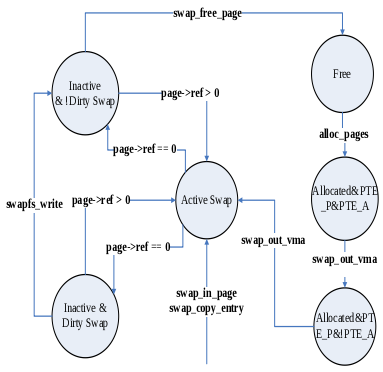
\includegraphics{figures/10.png}
\caption{9}
\end{figure}

ucore的物理页状态变化图

下面具体讲述一下proj11中实现上述置换算法的页面置换逻辑。在proj11中同时实现了积极换出策略和消极换出策略,这都是通过在不同的时机执行kwapd\_main函数来完成的。当ucore调用alloc\_pages函数以获取空闲页,但物理页内存分配器无法满足请求时,alloc\_pages函数将调用tre\_free\_pages来执行kwapd\_main函数(通过直接唤醒线程的方式,在lab3中会进一步讲解),完成对页的换出操作和生成空闲页的操作。这是一种消极换出的策略。另外,ucore设立了每秒执行一次kwapd\_main函数(通过设置timer来唤醒线程的方式,在lab3中会进一步讲解),完成对页的换出操作和生成空闲页的操作。这是一种积极换出的策略。

kswapd\_main是ucore整个页面置换算法的总控部分,其大致思路是根据当前的空闲页情况查找出足够多的可换出页(swap
page),然后根据这些可换出页的访问情况确定哪些是``常用''页,哪些是``不常用''页,最后把``不常用''的页转换成空闲页。思路简单,但具体实现相对复杂。

如前所述,swap 整个流程就是把尽可能多的 page 从变成
PG\_active的,并移动到 active list中;把 active list
中的页尽可能多的变成 inactive list 中页;最后把 inactive list
的页换出(洗净),根据情况处理洗净后的 page 结构(根据 page ref
以及相应的 dirty bit)。所以整个过程的核心是尽可能的断开页表中的 PTE
映射。

当 alloc\_pages 执行分配 n
连续物理页失败的时候,则会通过调用tree\_free\_page来唤醒kswapd线程,此线程执行kswapd\_main函数。kswapd
会发现它现在压力很大,需要尽可能的满足分配 n
个连续物理页的需求。既然需求是 n 个连续物理页,那么 kswapd
所需要释放的物理页就应该大于 n
个;每个页可能在某个或者许多个页表的不同的地方有 PTE 映射(特别是 copy
on write 之后,这种情况更为普遍),那么 kswapd 所需要断开的 PTE
映射就远远不止 n 个。Linux 实现了能够根据 physical address
在页表中快速定位的数据结构,但是实现起来过于复杂,这里 ucore
采用了一个比较笨的方法,即遍历所有存在的页表结构,断开足够多的 PTE
映射。这里足够多是个经验公式,采用 n\textless{}\textless{}5
。当然这也可能失败,那么 kswapd
就会尝试一定次数。当他实在无能为力的时候,也就放弃了。而 alloc\_pages
也会不停的调用 try\_free\_pages
进行尝试,当尝试不停的遭遇失败的时候,程序中会有许多句 warn
来输出这些调试信息。而 Linux
的方案是选择一个占用内存最多的进程杀掉并释放出资源,来尽可能的满足当前程序的需求(注意,这里当前程序是指内核服务或者调用),直到程序从内核态正常退出;ucore
的这种设计显然是过于简单了,不过此是后话。

扫描页表是一项艰巨的任务,因为除了内核空间,用户地址空间有将近 3G
的空间,真正的程序很少能够用这么多。因此,充分利用虚存管理能够很大的提升扫描页表的速度。

接下来,我们需要介绍一下 kswapd\_main 是如何一步一步完成 swap
的操作的。正如前面介绍的那样,swap 的任务主要分成三个过程,

现在我们来介绍以下 kswap\_main 是如何一步一步完成 swap
的操作的。正如前面介绍过的,swap
需要完成3件事情,下面对应的是这三个操作的具体细节:

\begin{enumerate}
\def\labelenumi{\arabic{enumi}.}
\item
  kswapd\_main函数通过循环调用函数swap\_out\_mm并进一步调用swap\_out\_vma,来查找ucore中所有存在的虚存空间,并总共断开
  m 个 PTE
  到物理页的映射(这里需要和进程的概念有所结合,可以理解为每个用户程序都拥有一个自己的虚存空间。但是需要提一句的是,在后的实验中还会遇到虚存空间在多个进程之间的共享;遍历虚存空间而不是遍历每个进程是为了避免某个虚存空间被很多进程共享进而被
  kswapd
  过度压榨所带来的不公平。可以想象,被过度压榨的虚存空间,同时又由于被很多进程共享从而有很高的概率被使用到,最终必然会导致频繁的
  \#PF,给系统不必要的负担。还有就是虽然 swap 的任务是断开 m 个 PTE
  映射,但是实际上它对每个虚存空间都一次至多提出断开 32
  个映射的需求,并循环遍历所有的虚存空间直到 m
  得到满足。这样做的目的也是为了保证公平,使得每个虚存空间被交换出去的页的几率是近似相等的。Linux
  实际上应该有更好的实现,它根据虚存空间所实际使用的物理页的个数来决定断开的映射的个数。)。这些断开的
  PTE 映射所指向的物理页如果没有 PG\_active 标记,则需要给他分配一个新的
  swap entry,并做好标记,将 page 插入到 active\_list 中去(同时也插入到
  swap 的哈希表中),然后设置好相应的 page\_ref 和 mem\_map{[}offset{]}
  的值,当然,如果找不到空闲的 swap entry 可以分配(比如 swap
  分区已经用光了),我们只能跳过这样的 PTE
  映射,从下一个地址继续寻找出路;对于原来就已经标记了 PG\_swap
  的物理页,则只需要完成后面的工作,即调整引用计数就足够了。断开的 PTE
  被 swap\_entry 取代,并取消 PTE\_P
  标记,,这样当出现\#PF的时候,我们能够直接根据 PTE
  上的值得到该页的数据实际是在swap 分区上的哪个位置上。

  现在不必要计较一个 page 究竟是放在 active\_list 还是放在
  inactive\_list 中,更不必要考虑换出这样的操作,这一阶段的工作只是断开
  PTE 映射,余下的工作后面会一步步完成。

  当 kswapd 断开足够数量的 PTE
  映射以后,这一部分的工作也就完成了。虚存管理中维护了一个 swap\_address
  的地址,表示上一次 swap 操作结束时的地址,维护这个数据是避免每次 swap
  操作都从虚存空间的起始地址开始,从而导致过多数量的重复的无效的遍历。

  当 kswapd 发现自己竭尽所能的遍历都无法满足断开 m
  个链接的需求时,该怎么办?我们需要明确的是swap
  操作的主要目的是释放物理页,而断开 PTE
  映射是一个必要的步骤,作用是尽可能的扩大 inactive\_list 中 page
  的个数,为物理页的换出提供更大的基数(操作空间),但并不是主要过程。所以为了防止在这一步陷入死循环,kswapd\_main
  最多会对全部虚存空间的链表尝试 rounds=16 次遍。
\item
  通过 page\_launder 函数,遍历
  inactive\_list,实现页的换出。这部分和下面 refill\_inactive\_list
  操作的先后顺序并不那么严格。通俗的解释就是 page\_launder 实现的是把
  inactive\_list 中的 page 洗净,并完成 page
  的释放,当然也顺便实现了把实际上活跃的(active) 的 page 从
  inactive\_list 上取下,放回 active\_list 的过程;而
  refill\_inactive\_list 从函数名上可以看出,实际上就是遍历
  active\_list,把实际上不活跃的(inactive) page 从 active\_list
  上取下,放到 inactive\_list 上,方便下一轮 page\_launder
  的操作。后者没有什么需要特别强调的,但是 page\_launder
  是比较复杂的过程,我们需要仔细的分析一下。page\_launder 先检查一个
  page 的 page\_ref 是否 != 0,如果满足,则表示该 page 实际上是 active
  的,则把它移动到 active\_list
  上去;如果不是,则需要对该页进行换出操作,过程如下:注意,下面讨论的是以
  page\_ref == 0 作为前提的。

  (*) page\_launder 的实现,涉及 ucore
  内核代码设计的一个重要假设前提,这是第一次涉及,以后的各个模块也会逐步大量涉及。这部分和进程调度又有一定的关联,提前了解一下,有助于理解这部分以后后续其它部分的代码。这个前提就是:ucore
  的内核代码是不可抢占的,也就是,执行在内核部分的代码,只要不是以下几种情况,通常可以认为是操作不会被抢占(preemption),即CPU控制权被剥夺。1.主动释放
  cpu 执行权限,比如调用 schedule 让其它程序执行;2.
  进行同步互斥操作,比如争抢一个信号量、锁;3.进行磁盘等等异步操作,由于
  kmalloc 有可能会调用 alloc\_pages 来分配页,而 alloc\_pages
  可能失败进而将cpu 让渡给 kswapd,所以,内核中的 kmalloc
  操作可以认为不是一个同步的操作。所有这样的非同步的操作一个可能的问题,就是所有执行比如
  kmalloc 这样的函数之前所做出的各种条件判断,在 kmalloc
  之后可能都不再成立了。

  你可以理解下面两段程序在运行时的差异,其中list
  是一个全局变量,并且可能被任何程序在执行内核服务的时候修改掉:

\begin{lstlisting}
parta:
if (!list_empty(list)) {
    ptr = (uintptr_t)kmalloc(sizeof(uint32_t));
    do_something(list_next(list), buffer);
    kfree(ptr);
}
partb:
ptr = (uintptr_t)kmalloc(sizeof(uint32_t));
if (!list_empty(list)) {
    do_something(list_next(list), buffer);
}
kfree(ptr);
\end{lstlisting}

  除此之外,中断处理的代码也需要进一步考虑进来。当内核尝试修改一部分数据的时候,如果该数据是中断处理流程可能访问的数据,那么内核需要对这次修改屏蔽中断;同理,如果中断处理需可能修改一部分数据,并且内核打算尝试读取该数据,那么内核需要对读操作屏蔽中断,等等。
\end{enumerate}

\begin{itemize}
\item
  如果一个页的 mem\_map 项也为0:前面已经讨论过 mem\_map 和 page\_ref
  之间的关系。如果此时,这个页的 mem\_map 项也为0,说明这个时候已经没有
  PTE 映射指向它们了,无论是物理页还是 swap
  备份页。那么这个页也就没有必要洗净了。可以直接释放物理页以及相应的
  swap entry 了。(同时记得处理 swap 有关的链表,以下不再赘述)
\item
  如果一个页的 mem\_map 项不为0,但是没有 PG\_dirty 标记:page
  数据结构里面有 PG\_dirty 标记,swap
  部分的代码根据这个标记来判断一个页是否需要被洗净(写到 swap
  分区上)。这个 PG\_dirty
  标记在什么情况下设置,我们稍后会讨论。这种情况可以等价为物理页上的数据和
  swap
  分区上的数据是一致的,所以不需要洗净该页,因为该物理页本身就已经足够干净了。所以可以安全的和(1)
  中的操作一样对该物理页进行释放。
\item
  如果一个页的确有 PG\_dirty 标记:表示该页需要被洗净。ucore
  这里的实现存在一个
  bug,最新的代码已经修复了这个bug,不过bug对于理解这段代码没有影响 。

  先清楚,洗净一个页,需要调用 swapfs\_write
  函数,完成将物理页写到磁盘上的操作。前面已经强调过,我们假设所有磁盘操作是异步IO。
  先明确一下,当前的状态,page\_ref=0 \&\&mem\_map!=0 \&\&
  PG\_dirty,那么写出的过程中就可能发生下面许多种可能的场景:

  \begin{itemize}
  \item
    swapfs\_write
    操作失败了。磁盘操作不像内存操作,它应该允许发生更多的错误。
  \item
    其它进程又访问到相应的数据页,前面提到过,因为 PTE
    已经被修了,所以会产生\#PF,内核会根据 PTE 的内容在 swap hash
    里面查找到相应的物理页,并将它重新插入到相应的页表中,并更新该 page
    的 page\_ref 和 mem\_map 的值。整个过程发生时,swapfs\_write
    还没有结束。那么当完成洗净一个页的操作时(写到swap 分区),swap
    部分的代码应该有能力检测出这种变化。也就是在 swapfs\_write
    之后,需要再判断 page\_ref 是否依然满足 inactive 的。
  \item
    和b类似,不过不同的是,这次对物理页进行的是一个写操作。操作完成之后,进程又将该
    PTE 指向的页释放掉了。那么当 swapfs\_write
    返回的时候,它面对的条件,可能就变成了 page\_ref=0 \&\&mem\_map=0
    \&\&PG\_dirty。它应该能够处理这个变化。
  \item
    和c类似,不同的是,该page有两个不同的 PTE 映射。那么在swapfs\_write
    操作之前,状态可能是 page\_ref
    =0\&\&mem\_map=2\&!PG\_dirty,那么当c中的情况发生以后,该物理页的状态就可能变成了
    page\_ref=0\&mem\_map=1\&PG\_dirty了。swap 应该能够处理这种变化。
  \end{itemize}
\end{itemize}

综上所述,page\_launder
部分的代码变得相对复杂很多。大家可以参照程序了解ucore
是怎么解决这种冲突的。 最后,提及一下那个 bug。因为 swapfs\_write
是异步操作,并且是对该 page 的操作,ucore
为了保证在操作的过程中,该页不被释放(比如一个进程通过\#PF,增加
page\_ref到1,然后又通过释放该page减少page\_ref到0,进而触发内核执行
page\_free 的操作),分别在 swapfs\_write 前后获得和释放该 page
的引用(page\_ref\_inc/page\_ref\_dec)。但事实证明,这种担心是多余的。理由很简单,当page\_launder
操作一个页的时候,该页是被标记 PG\_swap 的,这个标记一方面表示 page
结构中的 index有意义,另一方面也代表了,这样的 page 的释放,只能够由
swap 部分的代码来完成(参见 pmm.c 以及后面 shmem.c 的处理)。所以,swap
在操作该 page 的时候,不可能有程序能够调用free\_page释放该 page。

而相反的,mem\_map 是一个需要保护的数据。这个是产生 bug
的地方,有兴趣的同学可以去自己理解一下。

此外,可以翻阅一下涉及到 page\_ref 修改的 pmm
部分的代码,不难发现,当一个 page 从 PTE 断开的时候,也就是 page\_ref
下降的时候,内核会根据 PTE 上的硬件设置的 PTE\_D 来设置
PG\_dirty。其实这就足够了。因为 PG\_dirty
并不需要时时刻刻都十分的准确,只要在 swap 尝试判断该 page
是否需要洗净的时候,PG\_dirty 是正确的,就足够了。所以只需要保证每次
page\_ref 下降的时候,PG\_dirty 是正确的即可。除此之外,在对每个页分配
swap\_entry 的时候,需要保证标记
PG\_dirty,因为毕竟是刚刚分配的,物理页的数据还从来没有写出去过。

总结一下,页换入换出的实现很复杂,但是相对独立。并且正是由于 ucore
的内核代码不可抢占使得实现变得相对容易一些。只要是不涉及 IO
操作,大部分过程都可以认为处于不可抢占的内核执行过程。

\section{proj9.1:实现共享内存}\label{proj9.1ux5b9eux73b0ux5171ux4eabux5185ux5b58}

实现共享内存功能的目的是为将来(lab5中才需要)不同进程(process)之间能够通过共享内存实现数据共享。共享内存机制其实是一种进程间通信的手段。proj9/proj9.1完成了不同页表中(目前仅局限于父子进程之间,lab3才涉及)的虚拟地址共享同一块物理地址空间的功能。由于目前的实现仅限于有亲属关系的进程,这实际上意味着这些具有共享物理地址空间的虚拟地址空间也是相同的。

\subsection{相关数据结构}\label{ux76f8ux5173ux6570ux636eux7ed3ux6784}

这部分的具体实现工作主要在kern/mm/shmem.{[}ch{]}和其他一些文件中。根据前面的分析,我们知道在mm\_struct
层面上管理了基于同一个页表的vma集合,这些集合表示了当前可``合法''使用(即使没有对应的物理内存)的所有虚拟地址空间集合。当前的vma\_struct定义如下:

\begin{lstlisting}
struct vma_struct {
    struct mm_struct *vm_mm;
    uint32_t vm_start;
    uint32_t vm_end;
    uint32_t vm_flags;
    vma_entry_t vma_link;
};
\end{lstlisting}

这 个是proj9.1以前的 vma\_struct
结构定义。由于vma中并没有描述此虚拟地址对应的物理地址空间,所以无法确保不同页表中描述同一虚拟地址空间的vma指向同一个物理地址空间,所以不同页表间的内存无法实现共享。于是我们可以对vma\_struct增加下面两个域(field):

\begin{lstlisting}
struct shmem_struct *shmem;
size_t shmem_off;
\end{lstlisting}

shmem的作用是统一维护不同mm\_struct结构(即不同页表)中描述具有共享属性的同一虚拟地址空间的唯一物理地址空间。如果
vma-\textgreater{}flags 里面有 VM\_SHARE,就表示 vma-\textgreater{}shmem
有意义,他指向一个 shmem\_struct结构的指针。shmem\_struct结构定义如下:

\begin{lstlisting}
struct shmem_struct {
    list_entry_t shmn_list;
    shmn_t *shmn_cache;
    size_t len;
    atomic_t shmem_ref;
    lock_t shmem_lock;
};
\end{lstlisting}

shmem\_struct包含了list\_entry\_t结构的shmn\_list,此链表的元素是shmn\_t结构的共享页描述(包含某共享虚拟页的信息(page
或者 swap entry),为了维护起来简便,里面借用了页表的PTE描述方式,除了
PTE\_P
用来区分是否是一个物理页以外,没有任何其它权限标记,所以后面提到的 PTE
应该是带引号的),所以此链表就是用来存储虚拟地址空间的PTE集合,即此共享的虚拟地址空间对应的唯一的物理地址空间的映射关系。shmem\_ref指出了当前有多少进程共享此共享虚拟空间。shmn\_t是用来描述一段共享虚拟空间的信息,可理解为一个shmem
node结构,其定义如下:

\begin{lstlisting}
typedef struct shmn_s {
    uintptr_t start;
    uintptr_t end;
    pte_t *entry;
    list_entry_t list_link;
} shmn_t;
\end{lstlisting}

在这个结构中,entry保存了一块(4KB)连续的虚拟空间的PTE数组,可以理解为一个二级页表,这个页表最大可以描述4MB的连续虚拟空间对应的物理空间地址信息。entry
中的每一项用于保存 physical address \textbar{} PTE\_P 或者
swap\_entry。这样能最大限度节约内存,并且能很快通过entry项计算出
对应的struct page。
而list\_link是用来把自身连接属于同一shmem\_struct结构的域-shmn\_list链表,便于shmem\_struct结构的变量对共享空间进行管理。这样就可以形成如下图所示的共享内存布局:

\begin{figure}[htbp]
\centering
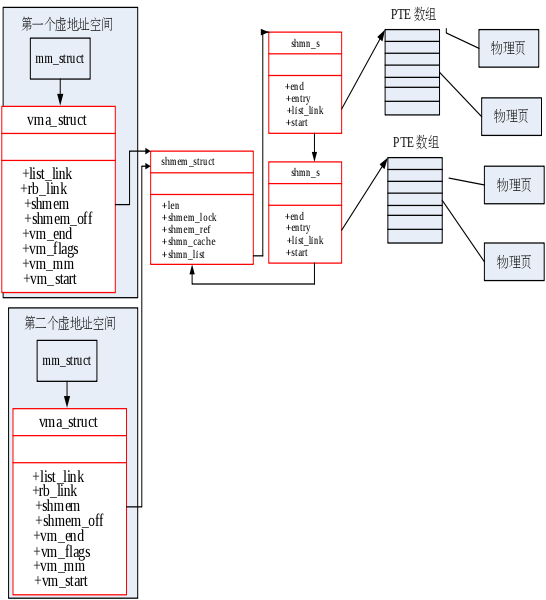
\includegraphics{figures/11.png}
\caption{11}
\end{figure}

\subsection{创建和访问共享内存的实现逻辑}\label{ux521bux5efaux548cux8bbfux95eeux5171ux4eabux5185ux5b58ux7684ux5b9eux73b0ux903bux8f91}

为了创建一块共享内存,首先需要在内核中调用do\_shmem函数(此函数要到lab3的proj12才会出现),do\_shmem函数并进一步调用shmem\_create函数创建一个shmem\_struct结构的变量,然后再调用mm\_map\_shmem函数来创建一个vma结构的变量,并设置vma的属性为VM\_SHARE,并把vma-\textgreater{}shmem指向shmem结构变量。这样就初步建立好了一个共享内存虚拟空间。

由于并没有给这块共享内存虚拟空间实际分配物理空间,所以在第一次访问此vma中某地址时,会产生缺页异(page
fault
),并触发do\_pgfault函数被调用。此函数如果发现是``合法''的共享内存虚拟空间出现的地址访问错时,将调用shmem的处理函数shmem\_get\_entry,来查找此共享内存虚拟子空间所在的其他虚拟地址空间中(具有不同的页表)是否此虚地址对应的PTE项存在,如果不存在,则表明这是第一次访问这个共享内存区域,就可以创建一个物理页,并在shmn\_s的entry中记录虚拟页与物理页的映射关系;如果存在,则在本虚拟地址空间中建立此虚地址对应的PTE项,这样就可以确保不同页表中的共享虚拟地址空间共享一个唯一的物理地址空间。

shmem结构中增加一个计数器,在执行复制某虚拟地址空间的copy\_mm函数的时,如果
vm\_flags 有 VM\_SHARE,则仅增加 shmem
计数器shmem\_ref,而不用再创建一个shmem变量;同理,释放
具有共享内存属性的vma
时,应该减少shmem计数器shmem\_ref,当shmem计数器shmem\_ref减少到0的时候,应该释放
shmem 所占有的资源。

另外,在shmem 里面不能记录地址,因为不同 vma
可能map到不同的地址上去,因此它只维护一个 page 的大小。上面提到的
shmem\_off 的作用是定位页面。具有共享属性的 vma 创建的时候,shmem\_off =
0。当 vma-\textgreater{}vm\_start
增加的时候(只可能变大,因为内核不支持它减小,unmap 的时候可能导致 vma
前面部分的 unmap,这就可能会让 vm\_start 变大),应该将 vm\_start
的增量赋给 shmem\_off,以保证剩下的 shmem
能够访问正确的位置。这样在访问共享内存地址addr发生缺页异常的时候,此地址对应的页在
shmem\_struct 里面的 PTE数组项的索引index 应该等于 (addr -
vma-\textgreater{}vm\_start + vma-\textgreater{}shmem\_off) / PGSIZE

\textbf{【注意】}

在页换出操作中, 尝试换出一页的条件是页的 page\_ref 到 0。为了防止 share
memory 的 page 被意外的释放掉,shmem
结构也会增加相应数据页的引用计数。那么对于一个share memory
的数据页,是不是就不能换出了?前面提到,页换出操作的第一步是扫描所有的虚拟地址空间,那么页换出操作就完全有能力知道当前扫描的
vma 是普通的 vma 还是对应的 share memory 的vma。正如 swap.c
里面看到的那样,swap 断开一个 page 以后,如果发现当前 vma 是share memory
的,并且 page\_ref 是1,那么可以确定的是这个最后一个 page\_ref 是在
shmem 结构中。那么swap 也同时将该 share memory 上的PTE 断开,就满足了
page\_launder 的换出条件。

share memory 上的 entry 换成了 swap entry
带来的坏处也很明显,因为标记share 的 vma
如果一开始没有页表内容,需要通过 \#PF 从shmem 里面得到相应的
PTE。但是不幸的是,得到的是 swap entry,那么只能再通过第二次
\#PF,才能将swap entry 替换成数据页。

\section{proj9.2:实现写时复制}\label{proj9.2ux5b9eux73b0ux5199ux65f6ux590dux5236}

proj9.2实现了写时复制(Copy On
Write,简称COW)的主要功能,为lab3高效地创建子进程打下了基础。COW有何作用?这里又不得不提前讲讲lab3中的子进程创建。不同的进程应该具有不同的物理内存空间,当用户态进程发出fork(
)系统调用来创建子进程时,ucore可复制当前进程(父进程)的整个地址空间,这样就有两块不同的物理地址空间了,新复制的那一块物理地址空间分配给子进程。这种行为是非常耗时和占内存资源的,因为它需要为子进程的页表分配页面,复制父进程的每一个物理内存页。如果子进程加载一个新的程序开始执行(这个过程会释放掉原来申请的全部内存和资源),这样前面的复制工作就白做了,完全没有必要。

为了解决上述问题,ucore采用一种有效的COW机制。其设计思想相对简单:父进程和子进程之间共享(share)页面而不是复制(copy)页面。但只要页面被共享,它们就不能被修改,即是只读的。注意此共享是指父子进程共享一个表示内存空间的mm\_struct结构的变量。当父进程或子进程试图写一个共享的页面,就产生一个页访问异常,这时内核就把这个页复制到一个新的页面中并标记为可写。注意,原来的页面仍然是写保护的。当其它进程试图写入时,ucore检查写进程是否是这个页面的唯一属主(通过判断page\_ref
和 swap\_page\_count 即 mem\_map 中相关 entry
保存的值的和是否为1。注意区分与share memory的差别,share memory 通过 vma
中的 shmem 实现,这样的 page 是直接标记为共享的,而不是 copy on
write,所以也没有任何冲突);如果是,它把这个页面标记为对这个进程是可写的。

在具体实现上,ucore调用dup\_mmap函数,并进一步调用copy\_range函数来具体完成对页表内容的复制,这样两个页表表示同一个虚拟地址空间(包括对应的物理地址空间),且还需修改两个页表中每一个页对应的页表项属性为只读,但。在这种情况下,两个进程有两个页表,但这两个页表只映射了一块只读的物理内存。同理,对于换出的页,也采用同样的办法来共享一个换出页。综上所述,我们可以总结出:如果一个页的PTE属性是只读的,但此页所属的VMA描述指出其虚地址空间是可写的,则这样的页是COW页。

当对这样的地址空间进行写操作的时候,会触发do\_pgfault函数被调用。此函数如果发现是COW页,就会调用alloc\_page函数新分配一个物理页,并调用memcpy函数把旧页的内容复制到新页中,并最后调用page\_insert函数给当前产生缺页错的进程建立虚拟页地址到新物理页地址的映射关系(即改写PTE,并设置此页为可读写)。

这里还有一个特殊情况,如果产生访问异常的页已经被换出到硬盘上了,则需要把此页通过swap\_in\_page函数换入到内存中来,如果进一步发现换入的页是一个COW页,则把其属性设置为只读,然后异常处理结束返回。但这样重新执行产生异常的写操作,又会触发一次内存访问异常,则又要执行上一段描述的过程了。

Page结构的ref域用于跟踪共享相应页面的进程数目。只要进程释放一个页面或者在它上面执行写时复制,它的ref域就递减;只有当ref变为0时,这个页面才被释放。


\section{小结}
缺